\section{Auswertung}
\label{sec:Auswertung}
%Hier kannst du ja noch einen Satz schreiben, wenn du möchtest xD
Für den Fehler $\Delta N$ der gemessenen Teilchen $N$ gilt
\begin{equation*}
    \Delta N = \sqrt{N} \,,
\end{equation*}
da radioaktive Zerfälle poissonverteilt sind.

\subsection{$\gamma$-Strahler}

Bei der zu Beginn über einen Zeitraum von $t = 900 \,\unit{\second}$ durchgeführten Nullmessung wurden
\begin{equation*}
    N_0  = 845 \pm 29
\end{equation*}
Ereignisse gemessen.
Das entspricht einer Ruheaktivität von
\begin{equation*}
    A_0 = (0.94 \pm 0.032) \,\dfrac{1}{\unit{\second}} \, .
\end{equation*}

In der \autoref{tab:gammablei} sind die Messdaten der ersten Messreihe, also mit Bleiplatten als Absorbermaterial, angegeben.
\begin{table}[H]
    \centering
    \caption{Messwerte zum $\gamma$-Strahler mit Bleiabschirmung.}
    \label{tab:gammablei}
    \begin{tabular}{S[table-format=2.2] S[table-format=5.0] S[table-format=3.0] S}
      \toprule
      {$D \mathbin{/} \unit{\milli\meter} $} & {$\text{Teilchenzahl}$} & {$\text{Zeit} \,t \mathbin{/} \unit{\second}$} &{$ \left(\text{A}- \text{A}_0 \right) \mathbin{/} \unit{\frac{1}{\second}}$} \\
      \midrule
       1.40   & 10708  & 100 & {$106,14   \pm 1,03$}  \\
       1.24  & 10348  & 100 & {$102,54   \pm 1,03$}  \\
       1.18  &  9906  & 100 & {$ 98,12   \pm 0,10$}  \\
       1.34  & 10048  & 100 & {$ 99,54   \pm 1,00$}  \\
       1.16  & 10071  & 100 & {$ 99,77   \pm 1,00$}  \\
       1.26  & 10430  & 100 & {$103,36   \pm 1,02$}  \\
       1.14  & 10182  & 100 & {$100,88   \pm 1,01$}  \\
      10.18  &  8357  & 200 & {$ 40,85   \pm 0,46$}  \\
      10.20  &  9043  & 200 & {$ 44,28   \pm 0,48$}  \\
      20.10  &  3375  & 200 & {$ 15,94   \pm 0,29$}  \\
      \bottomrule
    \end{tabular}
  \end{table}

Zunächst wird die Hintergrundaktivität von der gemessen Aktivität abgezogen.
Die so bereinigten Messdaten aus \autoref{tab:gammablei} werden in einem halblogarithmischem Diagramm aufgetragen und es wird, wie in \autoref{fig:plot1} zu erkennen, eine Ausgeleichsfunktion berechnet.

\begin{figure}[H]
    \centering
    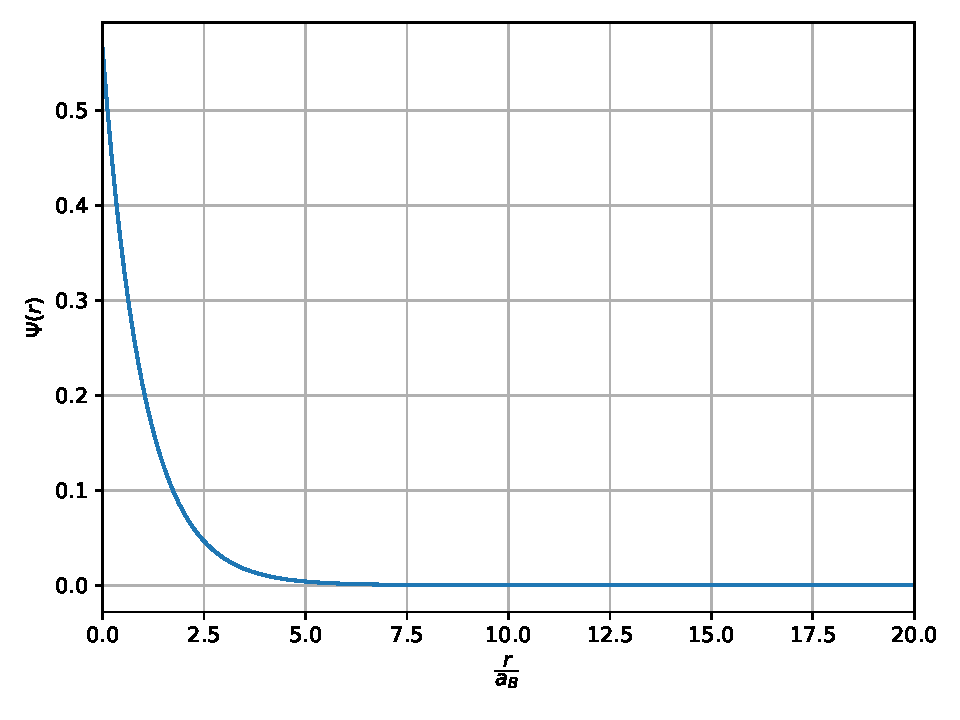
\includegraphics{Graph_a.pdf}
    \caption{Ausgeleichsfunktion zur Bestimmung des Absorptionskoeffizienten mit Bleiabsorber.}
    \label{fig:plot1}
  \end{figure}

Aus der Ausgleichsrechung wird der Absorptionskoeffizienten 
\begin{equation*}
    \mu =  \left( 96.958 \pm 5.079 \right) \mathbin{/} \unit{\meter}
\end{equation*}
abgelesen. 
Die Anfangsaktvität bzw. der y-Achsenabschnitt, ist mit 
\begin{equation*}
    A =  \left( 111.434 \pm 1.024 \right)  \dfrac{1}{\unit{\second}}
\end{equation*}
gegeben. \\

Analog wird für die zweite Messreihe verfahren.
Dabei sind in \autoref{tab:gammakupfer} die Messdaten für die unterschiedlichen Dicken der Kupferabsorber dargestellt.

\begin{table}[H]
    \centering
    \caption{Messwerte zum $\gamma$-Strahler mit Kupferabsorber.}
    \label{tab:gammakupfer}
    \begin{tabular}{S[table-format=2.2] S[table-format=5.0] S[table-format=3.0] S}
      \toprule
      {$D \mathbin{/} \unit{\milli\meter} $} & {$\text{Teilchenzahl}$} & {$\text{Zeit} \,t \mathbin{/} \unit{\second}$} &{$ \left(\text{A}- \text{A}_0 \right) \mathbin{/} \unit{\frac{1}{\second}}$} \\
      \midrule
       0.70           &      10948      &      100  	& {$108,54  \pm 1,05$} \\
       0.62           &      11137      &      100  	& {$110,43  \pm 1,06$} \\
       0.51           &      11065      &      100  	& {$109,71  \pm 1,05$} \\
       0.54           &      10953      &      100  	& {$108,59  \pm 1,05$} \\
       4.94           &      18462      &      100  	& {$183,68  \pm 1,36$} \\
      20.00           &       9863      &      200  	& {$ 48,38  \pm 0,50$} \\
      20.10           &      10257      &      200  	& {$ 50,35  \pm 0,51$} \\
      \bottomrule
    \end{tabular}
  \end{table}

  Erneut werden die aufgenommenen Ereignisse grafisch aufgetragen und es wird eine Ausgleichsrechung durchgeführt, sodass der in \autoref{fig:plot2} zu erkennende Plot entsteht.

  \begin{figure}[H]
      \centering
      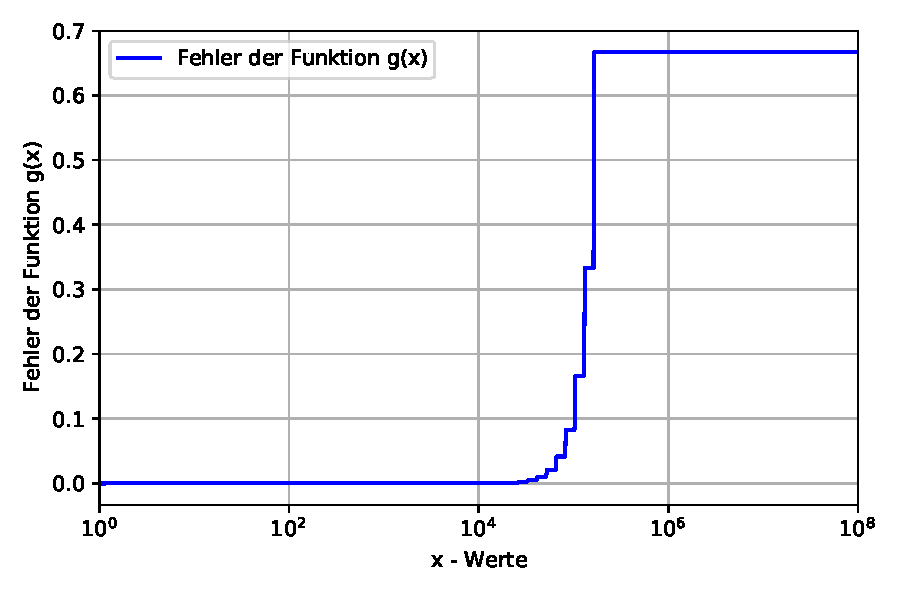
\includegraphics{build/Graph_b.pdf}
      \caption{Ausgeleichsfunktion zur Bestimmung des Absorptionskoeffizienten mit Kupferabsorber.}
      \label{fig:plot2}
  \end{figure}

Hier ergibt sich der Absorptionskoeffizient zu
\begin{equation*}
    \mu =  \left(33.484 \pm 22,824\right) \mathbin{/} \unit{\meter}
\end{equation*}
und die Anfangsaktivität zu
\begin{equation*}
    A = (4,827 \pm 0,153) \, \unit{\frac{1}{\second}}
\end{equation*}

Verglichen mit einem Theoriewert von % Hast du den Theoriewert irgendwo?

\begin{equation*}
    \mu_{\text{theo}} = ................
\end{equation*}

\subsection*{$\beta$-Strahler}

Mithilfe der in \autoref{tab:beta} dargestellten Werte Wird erneut eine Regressionsrechnung durchgeführt. 
\begin{table}[H]
    \centering
    \caption{Messwerte zum $\beta$-Strahler.}
    \label{tab:beta}
    \begin{tabular}{S[table-format=3.0] S[table-format=5.0] S[table-format=3.0] S}
      \toprule
      {$D \mathbin{/} \unit{\micro\meter} $} & {$\text{Teilchenzahl}$} & {$\text{Zeit} \,t \mathbin{/} \unit{\second}$} &{$ \left(\text{A}- \text{A}_0 \right) \mathbin{/} \unit{\frac{1}{\second}}$} \\
      \midrule
      {$482 \pm 1.0$}      &         339      &       500  &  0.035 \pm 0.005 \\
      {$444 \pm 2.0$}      &         335      &       500  &  0.027 \pm 0.004 \\
      {$400 \pm 1.0$}      &         338      &       500  &  0.033 \pm 0.004 \\
      {$338 \pm 5.0$}      &         293      &       400  &  0.089 \pm 0.011 \\
      {$302 \pm 1.0$}      &         324      &       400  &  0.167 \pm 0.013 \\
      {$253 \pm 1.0$}      &         228      &       300  &  0.117 \pm 0.018 \\
      {$200 \pm 1.0$}      &         655      &       300  &  1.540 \pm 0.053 \\
      {$160 \pm 1.0$}      &        1207      &       200  &  5.392 \pm 0.141 \\
      {$152 \pm 0.5$}      &        1957      &       200  &  9.142 \pm 0.189 \\
      {$125 \pm 0.0$}      &        1906      &       200  &  8.887 \pm 0.186 \\
      {$100 \pm 0.0$}      &        8006      &       200  & 39.387 \pm 0.415 \\
      \bottomrule
    \end{tabular}
  \end{table}

Wie in \autoref{fig:plot3} zu erkennen, wird dabei die Massenbelegung $R$ halblogarithmisch gegen die Aktivität $A - A_0$ geplottet.
\begin{figure}[H]
    \centering
    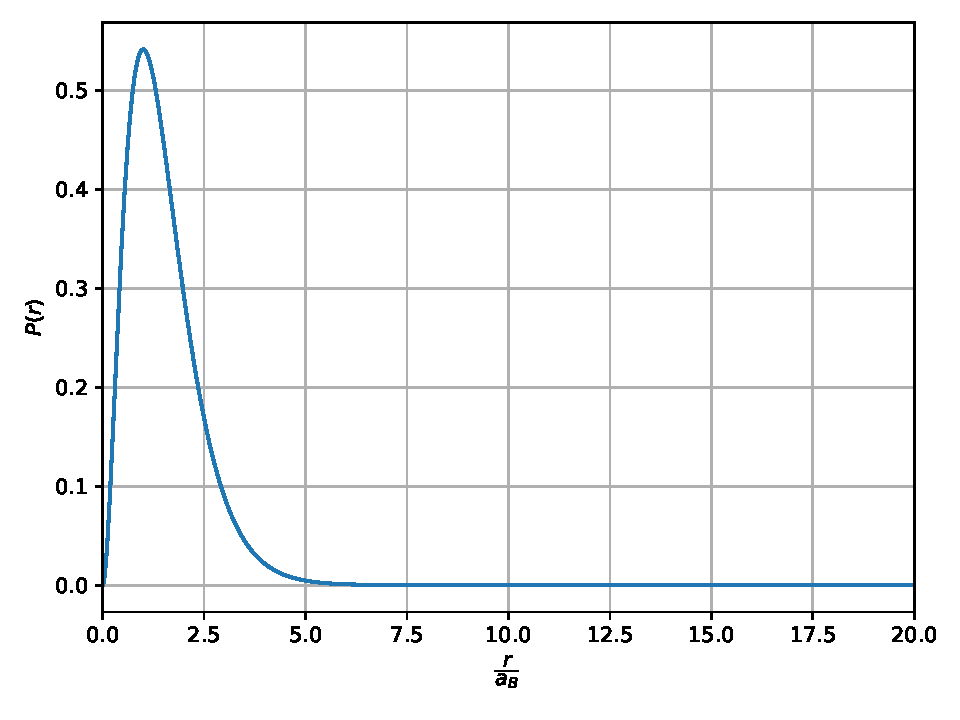
\includegraphics{build/Graph_c.pdf}
    \caption{Durchgehende Strahlungsintensität und Untergrundstrahlung in Abhängigkeit der Massenbelegung $R$.}
    \label{fig:plot3}
\end{figure}
Die beiden eingezeichneten Geraden stellen die durchgehende Strahlungsintensität sowie die Untergrundstrahlung dar. \\
Dabei ist die Gesamtreichweite $R_\text{max}$ der Strahlung durch
\begin{equation*}
    R_\text{max} = \frac{b_2 - b_1}{m_2 - m_1}
\end{equation*}
gegeben, wobei $b_i$ die y-Achsenabschnitte und $m_i$ die Steigungen der beiden Geraden repräsentieren. \\

Mit
\begin{align*}
    m_1 &= ... \\
    m_2 &= ... \\
    b_1 &= ... \\
\end{align*} ergibt sich
\begin{equation*}
    R_\text{max} = ......\, \unit{\meter} \,.
\end{equation*}
und damit nach \eqref{eq:Emax} eine Maximalenergie von
\begin{equation*}
    E_\text{max} = ...... \pm ..... \,\unit{\kilo\eV}
\end{equation*}


